% !TeX spellcheck = en_US
\section{Application overview}\label{section:overview}

In this chapter we will provide general overview of main application window.

\begin{figure*}[!ht] 
	\centering
	\makebox[\textwidth]{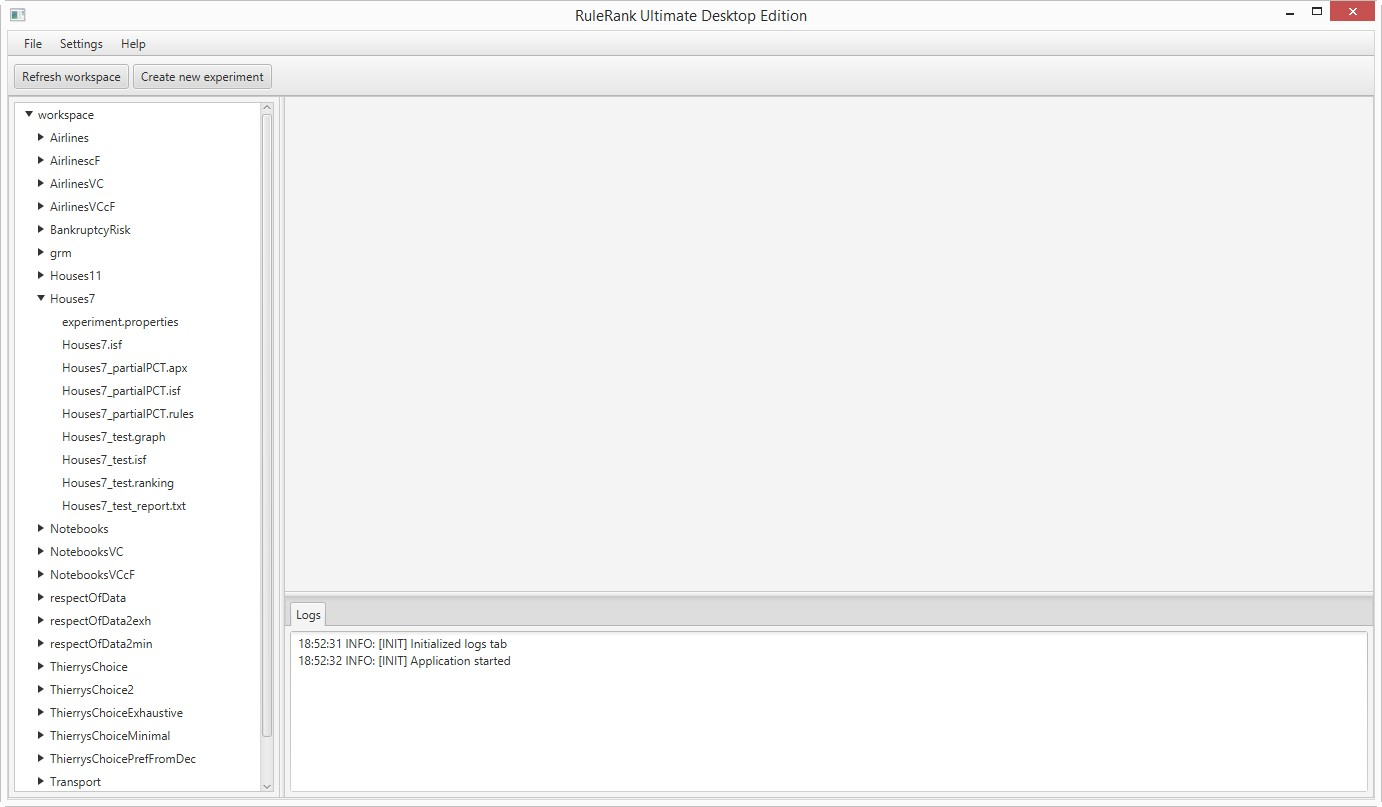
\includegraphics[width=.7\paperwidth]{overview}}
	\caption{Main window}
\end{figure*}

There are three main panels in RUDE application:
\begin{itemize}
	\item \textbf{workspace (1)} - it manages all files
	\item \textbf{upper panel (2)} - it displays most of the information. It can display multiple tabs like web browser. Most of the work will be done here.
	\item \textbf{lower panel (3)} - it contains logs and can display additional information for some upper tabs. It can display multiple tabs like web browser.
\end{itemize}

On top of main window you can find menu:
\begin{itemize}
	\item \textbf{File} - it currently enables to quit program
	\item \textbf{Settings} - it contains user settings for RUDE application
	\item \textbf{Help} - it contains About and Help modal dialogs.
\end{itemize}

Below menu you can find toolbar with actions, with will be described in \hyperref[section:workspace]{Workspace management section}.


\subsection{Tabs management}\label{sub:overview-tab}
New tab is created after opening file from workspace. You can do this by double clicking on file in workspace tree. Many tabs can be opened at once, but only one for each file. After pressing right click on tab header, you will see context menu containing actions with can close many tabs at once. If you made some changes in editable tab form, you will be asked for confirmation, if you try to close it by context menu action. Same confirmation appears when you try to exit application or close single tab.\\

Logs tab display all logs from application. 
Currently there are three logs levels:
\begin{itemize}
	\item \textbf{INFO} - displays some useful information about performed actions
	\item \textbf{WARN} - indicates some misconfiguration or action aborting in certain conditions. It also indicates errors handled by application.
	\item \textbf{ERROR} - displays errors not handled properly by application
\end{itemize}

Logs can be copied by selecting text and pressing Ctrl + C. All logs can be cleared by right clicking on logs panel and choosing ''Clear logs'' option.
\newline\newline
Next sections describes all application windows with are available for user.

\subsection{High level workflow}\label{sub:overview-flow}

This section provides high level steps for performing experiment. As a result of experiment, application will produce ranking of objects, from best to worse, basing on gain/cost criteria configured in isf tables and initial pairs comparison/ranking.

\begin{enumerate}
	\item Create experiment directory with will contain all experiment files.
	See \hyperref[section:workspace]{Workspace section}.
	\item Create learning data file (.isf) containing objects on with ranking will be created.
	See \hyperref[section:isf-table]{Isf edition section}.
	\item (Optional) Create test data file (.isf)
	See \hyperref[section:isf-table]{Isf edition section}.
	\item Create experiment properties file and configure experiment.
	See \hyperref[section:properties]{Properties section}.
	\item Create sample ranking or pairs comparisons in experiment properties form.
	See \hyperref[sub:properties-ranking]{Ranking configuration section},
	see \hyperref[sub:properties-pairs]{Pairs configuration section}
	\item Run experiment in properties form.
	See \hyperref[section:experiment-running]{Experiment running section}.
	\item See logs and generated files for experiment results.
\end{enumerate}

 Experiment will perform analysis using Dominance-based Rough Set Approach (DRSA) or Variable Consistency Dominance-based Rough Set Approaches (VC-DRSA) (depending on options selected).
 
 At first, it will generate Pairwise Comparison Table (PCT), where all objects are compared between each other on all criteria. Partial PCT table will be saved to .isf file, because full table is to big to save.
 See \hyperref[sub:pct-isf]{Partial comparison table section}.
 
 From pairwise comparison table dominance cones are calculated, with represents approximate outranking and non-outranking relations in PCT. Also some metrics are calculated. There are saved in text format to .apx file. 
 See \hyperref[sub:pct-apx]{Partial comparison table section}.
 
 In next step application induces rules from Pairwise Comparison Table. S relation indicates outranking relation, Sc indicates non-outranking relation. Rules can be certain or possible. Also rule statistics are generated and saved in .rules file next to induced rules. 
 See \hyperref[section:rules]{Rules section}.
 
 Next, preference graph is generated, in with nodes represents objects from isf table and arcs represents S or Sc relations. Arcs in graph can be also weighted, where weight represents satisfaction degrees of the preference relations. Weight for relation (arc) is calculated by aggregating confidence of covering rules. Preference graph is saved to .graph file.
 See \hyperref[section:graph]{Graph visualisation section}.
 
 As the last step, final ranking is calculated from preference graph. It contains objects positions and scores. Ranking is saved to .ranking file. In some cases also report can be generated and saved to .txt file.
  See \hyperref[section:ranking]{Ranking section}.
 
 
\vfill\newpage